\documentclass{article}


\title{Report}

\usepackage{graphicx}
\makeatletter
\newcommand{\verbatimfont}[1]{\renewcommand{\verbatim@font}{\ttfamily#1}}
\makeatother


\author{
	Trever Hallock \and
	Tamlyn Harley \and
	Matthew Stanley \and
	Cody Zhang
}

\begin{document}

\verbatimfont{\small}%

\maketitle

\abstract{
Simulation is an integral part of any mathematical modeling, especially when solving real-world problems.
Without a standard process to simulate solutions, those designing and implementing models would be unable to verify their efficacy.
Sam's Hauling requires an efficient method to schedule their drivers to service customer requests.
Currently this is done by hand, and our job was to assist other teams in creating algorithms to accomplish this task by simulating their results.
We developed a MATLAB model that took in a city object and a solution matrix to output the efficiency of said solution based on multiple metrics.
Also, we worked with the User Interface Team to translate between their Excel-based output and our MATLAB model.
Finally, we worked to find and simulate more subtle solution characteristics than what were explored by the other teams.
We produced a software package that was able to meet our goals and simulate the models given by the other teams involved.
}

\clearpage
\tableofcontents
\clearpage


\section{Introduction}

The Simulation Team's goals were to produce a reasonably efficient way to test solutions given by the other teams who were developing mathematicals models to solve Sam's Hauling's delivery scheduling.
We met our goals on time and created a software package that is not only robust but is capable of simulating many different situations and occurrences.

\subsection{Problem description}

Sam’s Hauling Inc. provides a small to medium sized dumpster rental service to customers in the Denver Metro Area.
They first deliver these dumpsters, or containers, to customers who fill them. Then Sam’s Hauling must return to collect the full dumpsters and take it to a dump for disposal.
Therefore, drivers must constantly be delivering new containers, picking up full containers, and dropping off trash at dumps.
There are also staging areas where drivers begin their day, and where empty dumpsters are stored.
These have capacities and initial inventories that must also be considered.
Currently, they schedule their drivers by hand, and are looking for a new method to optimally schedule their pickup and delivery routes.

\subsection{Overview of our role in the problem}

We created three pieces of software, using MATLAB, for other groups to use in testing their solutions:

\begin{itemize}
\item A city generator that will create random stops, dumps, and staging areas with which others can experiment
\item A simulation function that will simulate how well a solution satisfies several of these requests, and output its efficiency based on various metrics
\item A translate function that takes data from the User Interface team and transforms it into MATLAB
\end{itemize}

These three pieces of software have been used by the other teams in testing their proposed solutions.  Our goal was to provide an objective means by which others can efficiently test their proposed solutions, compare feasibility and optimality of said solutions, and give a good estimate of the sensitivity of each solution to changes - and we believe that we have met our goals.


As a group, our roles were diverse and varied; we all contributed to developing our software package in various aspects including coding, feature implementation, interface development, and style.  Individually, we all filled different roles in the end:

\begin{itemize}
	\item Trever Hallock
	\begin{enumerate}
		\item Coding (shared with Matthew Stanley)
		\item Reporting and documentation (shared with Tamlyn Harley)
	\end{enumerate}
	\item Tamlyn Harley
	\begin{enumerate}
		\item Testing and debugging the simulator function
		\item Reporting and documentation (shared with Trever Hallock)
	\end{enumerate}
	\item Matthew Stanley
	\begin{enumerate}
		\item Coding (shared with Trever Hallock)
		\item Team organization and scheduling
	\end{enumerate}
	\item Cody Zhang
	\begin{enumerate}
		\item Algorithm design and pseudocode
		\item Testing and debugging the city generator
	\end{enumerate}
\end{itemize}

Further features were developed as a team, and coded by Trever Hallock and Matthew Stanley; the final report was written by the entire team, and the testing of the finalized product and features were completed by Tamlyn Harley and Cody Zhang.


\subsection{Goals}

As a team, our objective was to create a software package that could simulate solutions through routes and cities to output their efficiency using various metrics.  
We did not set out with the goal of stating our opinion on whether these metrics were ``good" or ``bad," but instead simply reported the data to those using the software and allowed them the freedom to interpret the results independetly. 

We also had the objective of making our software user friendly; part of this was to allow easy translation between Excel (what the User Interface team ended up using) and MATLAB (our chosen platform).  This was a necessary goal in bridging the gap between the two platforms, and without this the teams would have to manually translate the information - which would be hardly "user friendly."  In the same vein as user friendliness, we also set out with the goal of creating a tutorial / manual for the class to use so that they could better understand the features and capabilities of our simulator.  This tutorial was completed and presented to the class as a whole, and was available for download along with our simulator.


\subsection{The Value of the Simulator}

Our software simulates the existing vehicle routing problems, except it also took inventory constraints on the containers in each staging area into account. It is a critical part of the solution because without the simulator, proposed solutions would not be as rigorously tested as they were. 

A working simulator was integral in allowing the others teams to test their proposed solutions and data to measure their efficiency and accuracy; without the simulator, this would have had to be done by hand. 

Our plan was to create a working software package as early as possible for every group to begin using, and we met this goal. 
A working version of the simulator was provided to the class on 30 October 2014, giving the class more than a month to work with the software to test their solutions.  Along with this, we also presented our tutorial.

Additionally, we hope that in the time remaining we can use the simulator gain a deeper understandning of the problem; test different assumptions made in the class, like constant drive times; be able to test solution robustness to changes in requests; and, possibly, even create an iterated solution method that attempts to solve the entire problem.

\section{MATLAB Model}

There are many parts to the model that we have created, as detailed below.

\subsection {MATLAB Object Model}


\subsubsection{City Representation}
Cities are objects that store multiple pieces of information. 
The city stores all of the data about drive times, stops, customer requests, landfills, staging areas, trucks, etc. 
It is an entire set of data that makes up the problem statement. 


\paragraph{Actions}
A city contains \emph{actions}, also called \emph{stops}.
There are multiple actions for any city.
An action is simply something a driver can do.
An action has several main parts:

\begin{description}
\item[The Operation ] \hfill \\
 This can be P (pickup), D (dropoff), R (replace), S (stage), U (unstage), or E (empty).
\item[The In-size   ] \hfill \\
 This is the size of the dumpster that is being brought to the action or stop, as a numerical value between of 0, 6, 9, 12, or 16.
The 0 represents no dumpster and the others represent the four sizes of containers we are dealing with.
\item[The Out-size  ] \hfill \\
 This is the same thing as in-size, but it is what size of dumpster the driver is supposed to leave with.
\item[The Start-time] \hfill \\
 This is the time, in seconds, when this action can start being performed; for example, if the start-time is 10,000, this means that 10,000 seconds must elapse during the simulation before this action can be performed.
\item[The Stop-time ] \hfill \\
 This is the time, in seconds, when an action must be performed by; together with start-time, these model time window constraints.
\item[The Wait-time ] \hfill \\
This is the amount of time it takes to actually complete the action (note that this is different from the travel time it takes to get to the location, which is modeled in a different place).
\item[The Location  ] \hfill \\
This is where the action is actually located; it is an index into the array of locations that we have, telling us which location has this particular action.
 It is also an index into the matrix of distances and durations between locations.
\end{description}


\paragraph{Example}

Different locations have different kinds of actions.
For example, staging areas have 8 actions each, as shown in this table:

\vspace{5mm}
\begin{tabular}{ | c | c | c | c |}
STAGING AREA & Operation & In-size & Out-size \\
\hline ACTION 1 & STAGE & 6 &  0 \\
ACTION 2 & STAGE & 9 &  0 \\
ACTION 3 & STAGE & 12 &  0 \\
ACTION 4 & STAGE & 16 &  0 \\
ACTION 5 & UNSTAGE & 0 &  6 \\
ACTION 6 & UNSTAGE & 0 &  9 \\
ACTION 7 & UNSTAGE & 0 &  12 \\
ACTION 8 & UNSTAGE & 0 &  16. \\
\end{tabular}

\vspace{5mm}



If you want to unstage (pickup) a size 12 dumpster, you must start with an empty truck and leave with a size 12 dumpster.
Thus, you would use the seventh action, which means your in-size is 0 and your out-size is 12.  
Having multiple actions is needed because only giving a location is ambiguous when a truck travels between staging areas.

Similarly, landfills have four actions each, one for each kind of dumpster you will be bringing there to empty.  
Customer requests only have one action each, as they will always have a predetermined in-size and out-size.
Now that we’ve covered cities, let us look at solutions.


\subsubsection{Solution Representation}

The the solution is represented by a matrix.
Each row represents a driver's route and each corresponding column entry a driver's row is what that driver will do in order.
A negative one means that the driver does nothing: he is at the end of his route.
The following is a solution matrix.

\vspace{5mm}

\[
\left(
\begin{array}{  c  c  c  c  c  c  c }
2 & 4 & 19 & 22 & -1 & -1 & -1  \\
10 & 17 & 19 & 44 & 11 & 13 & 5 \\
6 & 19 & -1 & -1 & -1 & -1 & -1  \\
\end{array} \right)
\]

\vspace{5mm}


Each row is a driver; thus, this city has three drivers.
Driver one performs action 2, then 4, then 19, then 22, and then he is done for the day.
Similarly, driver three performs actions 6 and 19, in that order, then finishes his day.  
Driver two is the busiest, obviously, but his actions are just as easily read.

As you can see, it was necessary to encode what kinds of dumpsters the driver was dropping off, picking up, etc. with the in-size and out-size, so that this matrix would be feasible. 
This encoding of the solution into a matrix is why there are so many actions associated with staging areas and landfills.
As an example, imagine that stop 19 is a staging area. 
Because of how the actions are structured, given any city, we will know exactly what kind of action the driver is performing at that staging area. 
Actions 18-25 may all be at that same staging area, but they all mean different things.


\subsection{Route Simulation}

\begin{verbatim}
   function [feasible, times, distances, num_serviced, fees, invs] 
      = simulate(c, sol, v, checkall)
\end{verbatim}

\paragraph{Parameters}
\begin{description}
\item[c] \hfill \\ The city object
\item[sol] \hfill \\ The solution matrix
\item[v] (Optional)\hfill \\   True if errors should be printed
\item[checkall] (Optional)\hfill \\  True if all constraints should be checked, even when one is violated
\end{description}

\paragraph{Return Values}
The simulate function takes in a city and a solution matrix as arguments, and outputs these metrics:

\begin{description}
\item[Feasible ]\hfill \\  False if the solution encountered an error that makes it a non-viable solution; it returns true otherwise
\item[Times ] \hfill \\ A vector containing all of the times it took each driver to complete his assigned route, based on the solution matrix given
\item[Distances ] \hfill \\ A vector containing all of the distances traveled by each driver based on his assigned route
\item[Number Serviced ] \hfill \\ How many of your customer requests were actually completed
\item[Fees ] \hfill \\ How much in fees you accrued on this route, based on the costs of landfills
\item[Inventories]\hfill \\  How many dumpsters remain at each staging area at the end of the day
\end{description}

Some solutions will contain errors that the simulator will recognize as non-feasible solutions. 
It will return the variable feasible = false if this is the case. 
Many things will cause it to return infeasible.
For example, if a driver visits a landfill followed by another landfill, this makes no sense and it will return infeasible.  
Or, if a driver visits a staging area to get a size 6 dumpster, but that staging area has none in inventory, this will also return infeasible.
If you want a detailed list of all the constraints refer to the matlab/src directory, or to the model in the next section.


Unless instructed otherwise, the simulator will continue to run to the best of its ability when dealing with a non-viable solution.
The errors it finds will be displayed in the main window of MATLAB.

Our suite of functions also comes with a generate\_rand\_solution function that takes a city as an argument.
However, beware, this random solution is rarely viable.



\subsection{City Generation}

\begin{verbatim}
   function [c] = generate_city(R, L, Y, D)
\end{verbatim}

The function generate\_city(R, L, Y, D) generates a city at random, based on these arguments:

\paragraph{Parameters}
\begin{description}
\item[R] The number of customer requests to be generated
\item[L] The number of landfills to be generated
\item[Y] The number of staging areas, or yards, to be generated
\item[D] The number of drivers that work in that city
\end{description}

\paragraph{Return Value}
\begin{description}
\item[c] A randomly generated city
\end{description}


This function creates a random set of customer requests, landfills, staging areas, trucks, etc. for us to run a simulation on.  Everything is random, so that you can create a diverse set cities to run simulations through. 


\subsection{City Translation}

\begin{verbatim}
   function [c] = translate(dirname)
\end{verbatim}

This function takes the output from the user interface team (who are working with Excel) and translates it into our city structure in MATLAB. 
It also finds the coordinateness of the addresses, to plot the city. 

For example, sample data given by the UI team on Canvas is also in our repository under /matlab/test/example\_ui\_data.
If you want a city based on this data, you can simply enter the matlab command c = translate('test/example\_ui\_data'); This city will represent the data found in this city.
Translate expects to see five files in the directory is given: output1.txt, output2.txt, output3.txt, output4.txt, and output5.txt.



Because this uses a Google API to find a location from the address the UI team gives, you must be connected to the internet to run this.

\section{Model}

(Needs to be integrated with previous section)


We will describe the mathematical model that this simulator attempts to simulate.

This includes detailing some of the assumptions that went into this model along with listing the parameters and variables for the model.

Finally, we will list the constraints and objectives.

\subsection{Model Assumptions}

Several assumptions were made to simplify the model.
For example, our model only takes trucks into account without worrying about drivers.
We see that drivers could be incorporated into the model be fixing a number of drivers and only letting this many trucks be anywhere but the start location at any given time.

Another assumption that went into our model is that when a costumer requests a certain size dumpster, the only feasible solutions are to give that costumer exaclty the dumpster that was requested.
This is more strict than the problem statement in which a large dumpster can be provided.

We provide arbitrary time windows that are more general than needed, because we only needed to have AM or PM time windows.
However we chose to include them in the model because Sam's Hauling mentioned that some customers do request pickups or delivers in specific time windows.

Also, drive times and wait times are assumed to be constant throughout the day.
This may or may not be a reasonable assumption.

We were not sure if we should include actions to be performed at staging areas that allowed drivers to dropoff a container and pickup a container in the same action.
We decided against this because this greatly increases the number of actions, solutions are required to first dropoff a dumpster and then pickup one up.



\subsection{Model Decisions}


\subsubsection{Cody's Idea}
\subsubsection{Modelling Language}
\subsubsection{Simulator output}

Somthing about no over simplying output for other teams (sum of times vs vector of times).
\begin{verbatim}

with sum + numdrivers^2 * max
driver costs: 
	
26259 26927 26691 25757 26812 26035 26599 26859 26848 26423 
times: 
	26259 26927 26691 25757 26812 26035 26599 26859 26848 26423 
	sum of all times: 265210

	max time: 26927
	
	
with sum
driver: 
	
    0     0     0 63056     0     0 24699     0 125832 41048 
times: 
	    0     0     0 63056     0     0 24699     0 125832 41048 
	sum of all times: 254635

	max time: 125832
	
	
with sum + overtime
driver: 
	
37924 37949 37922 38046 37941 37925 38064 37968 37942 37916 
times: 
	37924 37949 37922 38046 37941 37925 38064 37968 37942 37916 
	sum of all times: 379597

	max time: 38064

\end{verbatim}



\fbox{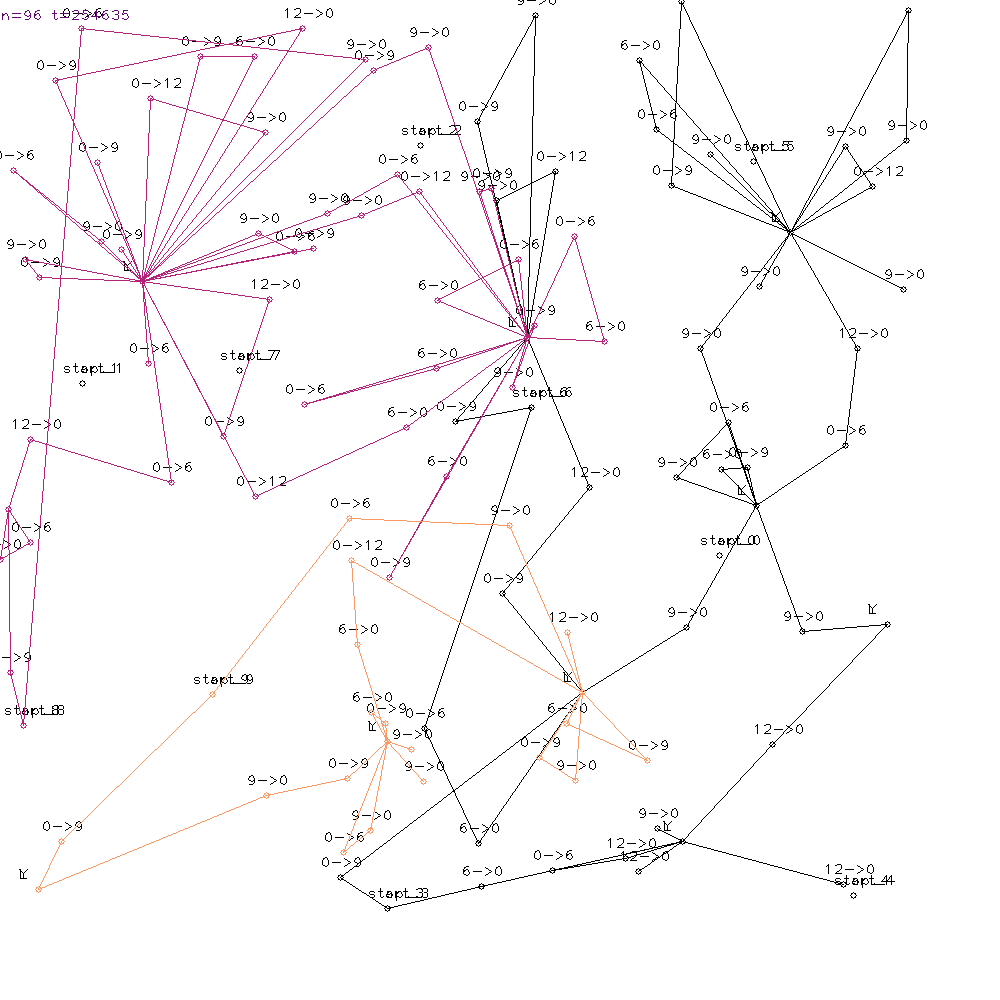
\includegraphics[width=6cm]{images/seed_0_sum.png}}
\fbox{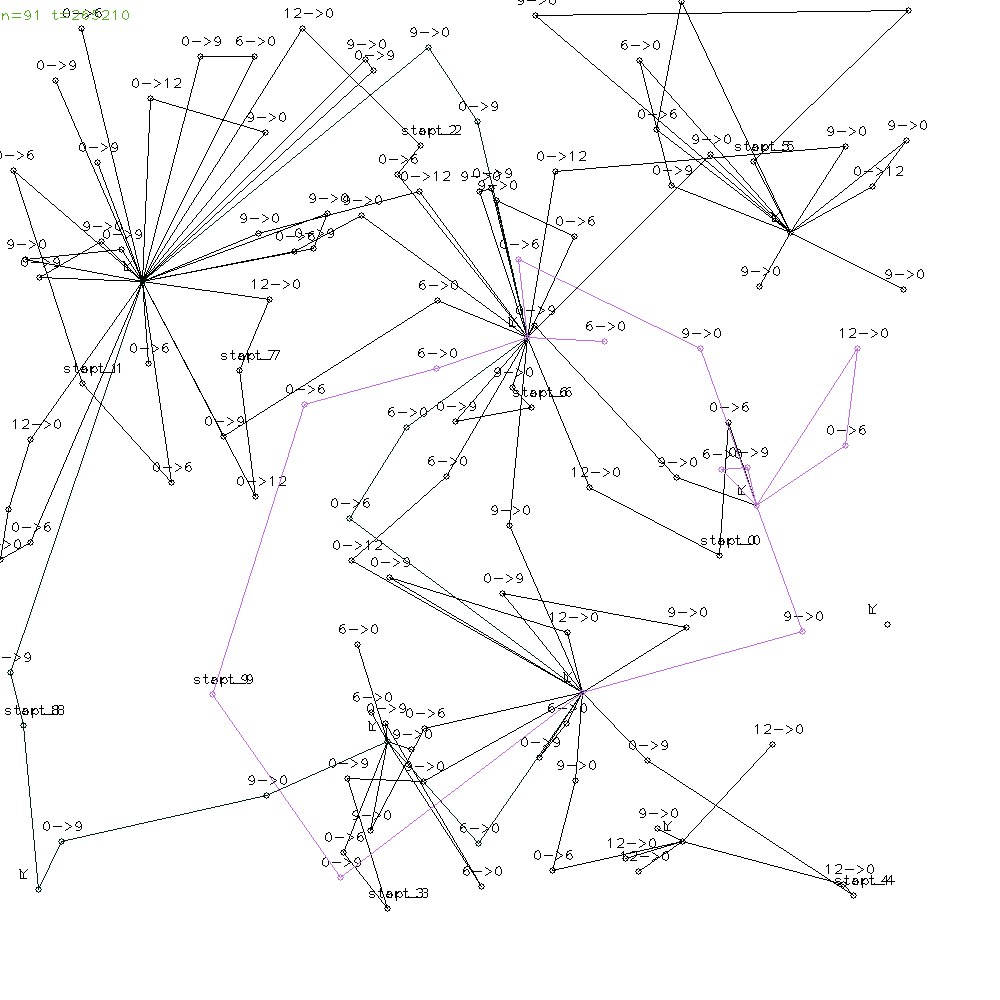
\includegraphics[width=6cm]{images/seed_0_max.png}}


\subsection{Model Variables}

First, we will define the variables used in the model.
While giving the symbols and their dimensions, we will try to use the following convention for indices.
For convenience, unless otherwise noted, 
$i$ will range from $1$ to $n$,
$j$ will range from $1$ to $m$,
$k$ will range from $1$ to $Y$,
$d$ will range from $1$ to $D$,
$t$ will range from $1$ to $|T|$,
and $l$ will be another index.
All times can be measured in seconds.



\subsubsection{Parameters}
\begin{tabular}{ l | l | l }
 Variable name                 &                                                                & Description                                                   \\
\hline
  $L$                          & $  L \ge 0                                                  $  & \# of Landfills                                               \\
  $Y$                          & $  Y \ge 0                                                  $  & \# of Staging Areas (or Yards)                                \\
  $R$                          & $  R \ge 0                                                  $  & \# of customer requests                                       \\
  $n$                          & $  n \ge 0                                                  $  & \# of actions, or stops                                       \\
  $m$                          &   $0 \le m \le n$                                              & \# of unique locations                                        \\
  $D$                          & $  D \ge 0                                                  $  & \# number of trucks (or Drivers)                              \\
  $S$                          &   For Sam's Hauling, $ |S| = 5$                                & Set of dumpster sizes                                         \\
                               & $                                                           $  & For Sam's Hauling, we will let                                \\
                               & $                                                           $  & S = \{                                                        \\
                               & $                                                           $  &   `6'                                                         \\
                               & $                                                           $  &   `9'                                                         \\
                               & $                                                           $  &   `12'                                                        \\
                               & $                                                           $  &   `16'                                                        \\
                               & $                                                           $  &   `No Dumpster'                                               \\
                               & $                                                           $  & \}                                                            \\
  $T$                          &   For Sam's Hauling, $ |T| = 3$                                & Set of possible Truck types                                   \\
                               & $                                                           $  & For Sam's Hauling, we will let                                \\
                               & $                                                           $  & T = \{                                                        \\
                               & $                                                           $  &  `small'                                                      \\
                               & $                                                           $  &  `medium'                                                     \\
                               & $                                                           $  &  `large'                                                      \\
                               & $                                                           $  & \}                                                            \\
  $O$                          & $  |O| = 6                                                  $  & Set of operations                                             \\
                               & $                                                           $  & O =\{                                                         \\
                               & $                                                           $  &  `D': deliver a dumpster                                      \\
                               & $                                                           $  &  `P': pickup a dumpster                                       \\
                               & $                                                           $  &  `R': replace a dumpster with a different one                 \\
                               & $                                                           $  &  `E': throw away a dumpster at a landfill                     \\
                               & $                                                           $  &  `S': Stage a dumpster                                        \\
                               & $                                                           $  &  `U': Unstage a dumpster                                      \\
                               & $                                                           $  & \}                                                            \\
%  $T_{max}$                    & $  T_{max}   \ge 0                                          $  & Total time in a day.                                          \\
%                               & $                                                           $  & Solutions that take more time are infeasible.                 \\
% \hline
%                               & $                                                           $  &                                                               \\
\end{tabular}


\subsubsection{The City}
\begin{tabular}{ l | l | l }
 Variable name                 &                                                                & Description                                                   \\
 \hline
  $I$                          & $ 1 \le I \le m, I \in \{s_k\}_{k=1}^Y                      $  & The starting index of all trucks.                             \\
                               & $                                                           $  &                                                               \\
                               & $                                                           $  &                                                               \\
                               & For each stop                                                  &                                                               \\
  $(T^{begin}_i, T^{end}_i)$   & $  1 \le i \le n, 0\le T^{begin}_i< T^{end}_i               $  & Time windows when stop $i$ is possible                        \\
  $W_i$                        & $  1 \le i \le n                                            $  & The wait time required to visit stop $i$                      \\
  $o_i$                        & $  1 \le i \le n                                            $  & Operation to be performed at stop $i$                         \\
  $(S^{in}_i, S^{out}_i)$      & $  1 \le i \le n                                            $  & The in and out dumpster sizes of each action.                 \\
                               & $                                                           $  & For example, if $o_i = $`S', then $S_i^{out} = $ No Dumpster  \\
  $l_i$                        & $  1 \le i \le n, 1 \le l_i \le m                           $  & The locations associated with each stop                       \\
  $c_{i,t}$                    & $  1 \le i \le n, 1 \le t \le |T|                           $  & Constraints on truck size                                     \\
                               & $  c_{i,t} \in \{0, 1\}                                     $  & 1 if action $i$ is accessible by truck type $t$               \\
                               & $                                                           $  & For example, we would like to set $c_{i,t} = 0$               \\
                               & $                                                           $  & when $o_i = 'R'$ and $S^{out}_i = '16'$                       \\
% \hline
                               & $                                                           $  &                                                               \\
                               & $                                                           $  &                                                               \\
                               & For each location                                              &                                                               \\
  $t_{j,l}$                    & $  1 \le j, l \le m, d_{i,j} \ge 0                          $  & Time duration to get from location $j$ to location $l$        \\
  $d_{j,l}$                    & $  1 \le j, l \le m, f_{i,j} \ge 0                          $  & Distance, between location $j$ to $l$ \\
% \hline
                               & $                                                           $  &                                                               \\
                               & $                                                           $  &                                                               \\
                               & For each truck                                                 &                                                               \\
  $t_d$                        & $ 1 \le d \le D, t_i \in T                                  $  &  Truck type of truck $d$                                      \\
% \hline
                               & $                                                           $  &                                                               \\
                               & $                                                           $  &                                                               \\
                               & For each staging area                                          &                                                               \\
  $I_{k, s}$                   & $ 1 \le k \le Y, s \in S \setminus \{\mbox{`No Dumpster'}\} $  &  Initial \# of dumpsters starting out in staging area $k$     \\
                               & $                                                           $  &  This is at the beginning of the day.                         \\
  $C_k$                        & $ 1 \le k \le Y, C_k \ge 0                                  $  &  \# of dumpsters that can fit into staging area $k$           \\
                               & $                                                           $  &  This stands for its Capacity.                                \\
                               & $                                                           $  & Obviously, $\sum_{j \in S} I_{k,j} \le C_k$ for each $k$      \\
  $s_k$                        & $ 1 \le k \le Y, 1 \le s_i \le m                            $  & location associated with staging area $k$                     \\
% \hline
                               & $                                                           $  &                                                               \\
                               & $                                                           $  &                                                               \\
                               & For each Land fill                                           &                                                               \\
  $F_l$                        & $  1 \le l \le L                                            $  & The fee associated with landfill $l$                          \\
  $e_l$                        & $1 \le e_l \le m, 1 \le l \le L                             $  & The location of landfill $l$                                  \\ 
\end{tabular}
\subsection{Other thoughts}

In matlab, the parameters 
  $L$,
  $Y$,
  $R$
will be required to generate a random city in addition to several distribution parameters.
A `city' will be encapsulated by the rest.

There are $R$ different actions to represent the requests, because there is only one action associated to each.
Then each dumpster size will have its own action for each landfill: one action where the in and out size is each dumpster size.
Then, for each staging area there will be actions allowing a dumpster to come in with no dumpster all leave with each dumpster size.
Also, there will be an action coming in to each staging area with each dumpster size and leaving with no dumpster.
That is, $n = R + (L + 2 Y) (|S| - 1)$.

\subsection{Decision variables}

The solution to the problem will be given by a matrix with $D$ rows and an arbitrary number of columns.
Each row $x_d, 1 \le d \le D$ will be a permutation vector of the stops to be performed by driver $d$ (followed by $-1$'s).
Let us name their lengths $r_d := length(x_d) \le n$.
We will interpret the $l$-th element of $x_{d}$ (which is denoted $x_{d,l}$) as the $l$-th stop to be performed by truck $d$.
For example, if $o_{x_{d,l}} =$ `S', then the $l$-th stop by driver $d$ is a staging operation at a storage yard.

\subsection{Objectives}

Let us make some of the following equations simpler with these definitions.
Let $t(x,y) = t_{x,y}$, so we have fewer subscripts.
For convenience of later sections, let us define a function $a(d, k)$ that represents the accrued time that truck $d$ takes to complete its $k$-th stop.
(We have assumed that $1 \le d \le D$, $1 \le k \le r_i$.)
This is given by:
$$a(d,l) := t(I, x_{d, 1}) + \sum_{j=1}^{l} W_{x_{d,j}} + \sum_{j=1}^{l-1} t(l_{x_{d,j}},l_{x_{d,j+1}} ).$$
That is, the time from the start location plus the times to travel between the stops, plus the time at each stop.

We will simulate this as a multi objective problem.
In revision one, this will only include the number of requests serviced, the time taken to do so, the total distance covered, and the amount of fees accrued.
We could use a lexicographic ordering to order these (If we have a maximum time).

\subsubsection{Number of requests serviced}

The total number of requests serviced is 
%either
%$$N = (\sum_{d=1} ^D \sum_{j=1 \atop o_j \in \{\mbox{`D'},\mbox{`P'}\}}^{r_d} 1) + (\sum_{i=1} ^D \sum_{j=1\atop o_j = \mbox{`R'}}^{r_d} 2)$$
%or
$$N = \sum_{d=1} ^D \sum_{j=1\atop o_j \in \{\mbox{`D'},\mbox{`P'}, \mbox{`R'}\}}^{r_d} 1.$$
%depending on whether servicing a replace request counts as twice the number of requests serviced as a pickup or delivery.

\subsubsection{Time taken to service requests}

One way to model the total time could be
$$ T_{total} = \max_{d=1} ^D \{ a(d, r_d) \} $$ which is the time of the longest route and would represent the amount of time before all routes were completed.
Another is to represent the total number of man-hours spent, which would instead be a sum of all times:
$$ T_{total} = \sum_{d=1} ^D  a(d, r_d)  .$$

It would be better to simply calculate the difference at each stop and its time window, 
and try to minimize the errors (or customer wait times/early inconveniences).
What the simulator will likely do is return an entire vector of time-costs associated with each driver.

If we also include fuel costs (or driving distances) between different locations, then another output will be the total distance driven.
Finally, if this is specifically fuel costs (and not driving distance) and we include the landfill fees, we could simply add the fees to driving costs and return it as an objective.

\subsubsection{Distance Covered}
This is given by
$$\sum_{d=1}^D d(I, x_{d, 1}) + \sum_{j=1}^{l-1} d(l_{x_{d,j}},l_{x_{d,j+1}} ).$$

\subsubsection{Landfill Fees}
This is given by

\[
\sum_{d=1}^D \sum_{j=1}^{r_d }
\{ \begin{array}{ccc}
 0 & \mbox {if } & o_{x_{d,j}}  \ne \mbox{`E'} \\
 F_l & \mbox{where } & e_l = l_{x_{d,j}} \\
\end{array}
\]


\subsubsection{Dumpster sizes}
This is future work, and might be used to ensure that dumpsters are equally (or otherwise) spread out among staging areas at the end of the day.
This could be used to ensure that dumpsters at staging areas are accessible for the next day.
Also, it is mentioned in the problem description that some staging areas might not be allowed to have dumpsters overnight.
Although we would need another parameter in the model to dictage which staging areas these are, that would likely make this objective be a constraint.

\subsection {Constraints}

\subsubsection{Permutations must not overlap}
We don't want to visit the same request twice, so for all $1 \le d, d' \le D$ and all $1 \le j, j' \le r_i$, at least one of the following $4$ statements must be true:

\begin{tabular}{ l r  c  l }
1: & $ d=d'$ & and & $j = j'$ \\
2: & $ o_{x_{d,j}}$ & $\in$ & $\{E, S, U\}$ \\
3: & $ o_{x_{d',j'}}$ & $\in$ & $\{E, S, U\}$ \\
4: & $x_{d,j}$ & $\ne$ & $x_{d', j'}$ \\
\end{tabular}

\subsubsection{Time for each stop falls within windows}
For each $1 \le i \le D$ and each $1 \le k \le r_i$ we need
$$ T^{begin}_{x_{i,k}} \le a(i, k) \le  T^{end}_{x_{i,k}}.$$

If we include the $T_{max}$ variable, we will need to ensure that $a(d,r_d) \le T_{max}$ for all $1 \le d \le D$

\subsubsection {Sizes match}

For all $1 \le d \le D$, and for all $1 \le j \le r_d - 1$, we have
$$S^{out}_{x_{d,j}} = S^{in}_{x_{d,j+1}}.$$
For all $1 \le d \le D$, we have
$$S^{in}_{x_d,1} = \mbox{`No Dumpster'} $$
as an initial constraint.

These mean that if a truck leaves a stop with a 9 dumpster, then he arrives at the next location with a 9x9 dumpster.
We also assume that all trucks start out with no dumpsters.

In the problem description, there is a statement that dumpsters larger than the one being requested can also be used.
We have not incorporated this into our model yet.

\subsubsection {Operations follow each other}
(Yes, this is needed! But wouldn't be if we instead used a dumpster state of full, or empty (which isn't the same as no dumpster) for each stop/action.
Then we would just need a `truck state matches' constraint, which would be as simple as the `sizes match' constraint.)

For all $1 \le d \le D$, and for all $1 \le j \le r_i - 1$, we need that $follows(o_{d, j}, o_{d, j+1})$ is true, where the $follows$ predicate has the following truth table:

\begin{tabular}{ c | c c c c c c }
 $follows$    & `D' & `P' & `R' & `T' & `S' & `U' \\
 \hline
 `D'          & F   & F   & F   & T   & F   & T   \\
 `P'          & T   & F   & F   & F   & T   & F   \\
 `R'          & F   & F   & F   & T   & F   & T   \\
 `T'          & F   & T   & T   & F   & F   & F   \\
 `S'          & F   & F   & F   & T   & F   & T   \\
 `U'          & T   & F   & F   & F   & T   & F   \\
\end{tabular}

Read this as operation in row $d$ can follow the operation in column $j$ if $follows(i,j) = $ T.

\subsubsection{Constraints on Truck Types}

For each $ 1 \le d \le D$ and each $1 \le j \le r_d $
we need $$ c_{x_{d,j},t_{d}} = 1 .$$

\subsubsection{Staging Area Capacities Met}

Let $b(d,t) $ ($b$ for bound) be the largest index $k$, $1 \le k \le r_i$ such that $a(d, k) < t$.
In other words, this is the a index into the $d$-th truck's route that gives its last stop before time $t$ ($t \in R$, $0 \le t < \infty $).

Then, we want that for each $1 \le y \le Y$, and each $s \in S \setminus \{\mbox{`No Dumpster'}\}$, and each $t \in R, 0 \le t < \infty $,

$$0 \le I_{y, s} 
 + \sum_{d=1}^D \sum^{b(d,t)} _{j=1 \atop { o_{x_{d,j}}  = \mbox{`U'} \atop   { S^{out}_{x_{d,j}} = s  \atop  s_y = l_{x_{d,j}}  }      }} (-1)
 + \sum_{d=1}^D \sum^{b(d,t)} _{j=1 \atop { o_{x_{d,j}}  = \mbox{`S'} \atop   { S^{in }_{x_{d,j}} = s  \atop  s_y = l_{x_{d,j}}  }      }} ( 1) \le C_i.$$
 
This assumes that each dumpster takes up the same amount of space in the staging area.
If not, we could use a weighted sum, where we replace the $\pm 1$ with a weight based on $s$
(the coefficients would need to be another parameter to the model).

\subsubsection{Each truck ends where it starts}
There is a constraint that says each truck must stop at the staging area it starts at.
That is, for all $1 \le d \le D$, we have $l_{x_{d, r_d}} = I$.

\subsection{Example}

%\subsection{TODO}
%Add the variable names next to their descriptions.
%Make more complicated examples.
%Add distances, and fees.


This is an example city with $L = 1$, $Y = 1$, $R = 2$, $D = 2$, $S = \{ \mbox{9  }, \mbox{12   }, \mbox{16   }, \mbox{No Dumpster} \}$,
$T = \{ \mbox {small}, \mbox{large}  \}$, $n=11$, $m=4$.

\subsubsection{City}
Possible Stops:

\begin{tabular} {c | c c c c c c c }
 index  & window begin & window end & wait time & operation & in size      & out size       & location  \\
\hline
   1    &    0         & 100        & 5         & `T'       & 9            & 9              &    1      \\
   2    &    0         & 100        & 5         & `T'       & 12           & 12             &    1      \\
   3    &    0         & 100        & 5         & `T'       & 16           & 16             &    1      \\
   4    &    0         & 100        & 2         & `U'       & No Dumpster  & 9              &    2      \\
   5    &    0         & 100        & 2         & `U'       & No Dumpster  & 12             &    2      \\
   6    &    0         & 100        & 2         & `U'       & No Dumpster  & 16             &    2      \\
   7    &    0         & 100        & 2         & `S'       & 9            & No Dumpster    &    2      \\
   8    &    0         & 100        & 2         & `S'       & 12           & No Dumpster    &    2      \\
   9    &    0         & 100        & 2         & `S'       & 16           & No Dumpster    &    2      \\
  10    &    0         & 50         & 1         & `R'       & 9            &        16      &    3      \\
  11    &    0         & 100        & 1         & `D'       & 16           & No Dumpster    &    4      \\
\end{tabular}


Truck Types:

\begin{tabular} {c | c c}
index & starting location   & type  \\
\hline
  1   &  2                  & small \\
  2   &  2                  & large \\
\end{tabular}

Distances:

\begin{tabular} { c c c c }
0  & 1  & 3 & 2 \\
1  & 0  & 2 & 4 \\
3  & .5 & 0 & 1 \\
2  & 1  & 3 & 0 \\
\end{tabular}

Constraints:

\begin{tabular} {c | c   c   c }
index     &    small   &   large \\
\hline
  1       &    1       &      1 \\
  2       &    1       &      1 \\
  3       &    0       &      1 \\
  4       &    1       &      1 \\
\end{tabular}

Staging areas:

\begin{tabular} {c c c }
index     &   capacity & location \\
 0        &     10     &    1     \\
\end{tabular}

$I = 6$.


\subsubsection{Solution}

These following two are possible solutions, although the second doesn't end where it starts.
1. $x_1 = ()$, $x_2 = ()$ (In this case, $r_1 = r_2 = 0$).
2. $x_1 = ()$, $x_2 = (6, 11, 4, 7)$ (In this case, $r_1 = 0$, $r_2 = 4$).

However, this solution is not feasible, because the sizes don't match in the last stop of the second truck:
$x_1 = ()$, $x_2 = (6, 11, 4, 8)$ (In this case, $r_1 = 0$,$ r_2 = 4$).

\subsubsection{Objective Values}

The time for the first is $0$, which is also the number of requests serviced.
The number of requests serviced in the second is $1$, and the time for the second truck $a(2, 4)$ is:
$$d_{l_6,l_6} + W_6 + d_{l_6,l_{11}} + W_{11} + d_{l_{11}, l_4} + W_{4} + d_{l_4,l_7} + W_7$$
$$ = d_{2,2} + W_6 + d_{2,4} + W_{11} + d_{4, 2} + W_{4} + d_{2,2} + W_7$$
$$ = 0 + 2 + 4 + 1 + 1 + 2 + 0 + 2 $$
$$ = 12. $$
Thus, $T_{total} = 12$ as well.



\section{Simulator}


\subsection{Performance}

Currently, the two most expensive functions of the simulator are the check that inventory bounds are satisfied and a helper function that computes the times each request is performed.
Which of these methods is most time consuming depends on how close to valid the solution is.

(Better graphics coming, but the one on the left is when the solution is not close to valid, while the one on the right is when all checks are performed.)

\fbox{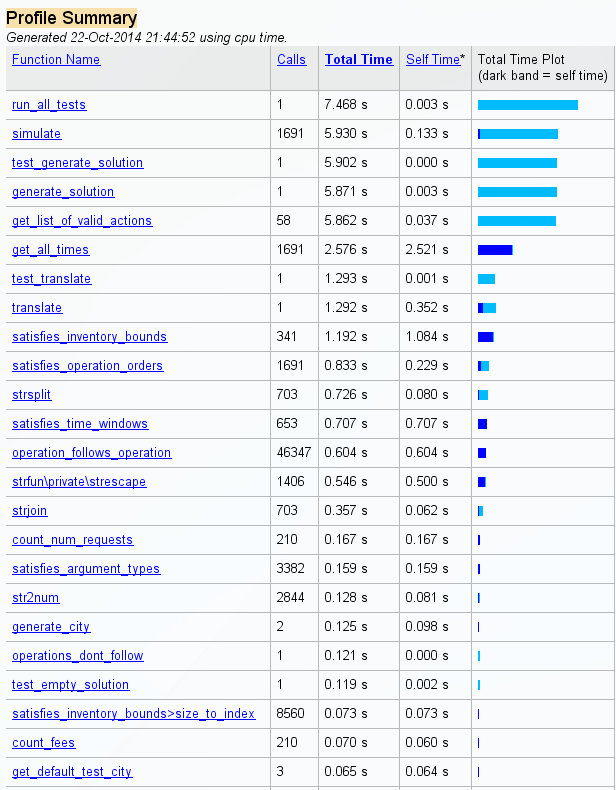
\includegraphics[width=5cm]{images/times_for_solutions_not_close_to_valid.png}}
\fbox{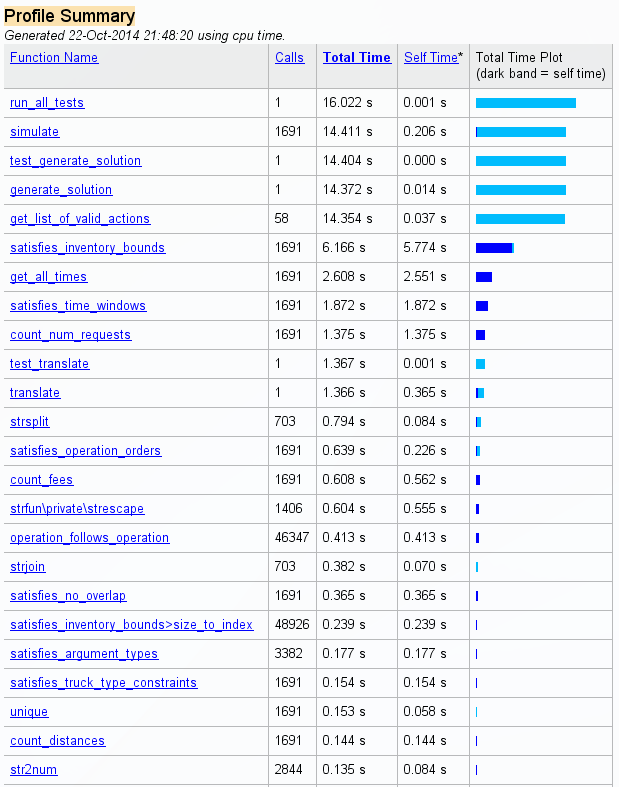
\includegraphics[width=5cm]{images/times_for_solutions_with_full_check.png}}

\subsection{Capabilities}

It was kind of sad that the capabilities section was empty.
Its not now.


\subsection{Failed attempts/Lessons learned}


\subsubsection{No way to express waiting}

We initially created the simulator without the ability to have a driver wait without performing any action;
this caused a problem because drivers were not able to wait for a time window to begin.  


\subsubsection{Identifying what needs to be remembered at stop}
Having locations in a solution was not not enough.

Additionally, we learned that each location must have multiple actions associated with them, 
as many things can be done at each location - an assumption we had not initially considered.


\subsubsection{Matrix dimension}
Some drivers did not have the same number of actions assigned to them, even if they took the same amount of time or longer than a driver with more actions.
We learned that less stops did not necessarily mean less productivity or efficiency.

When first creating a solution matrix, our assumption was that the matrix would always be size DxN, where D was the number of drivers in the city and N was the number of actions possible in the city. 
This turned out to be false because drivers could repeat actions, meaning that the matrix dimenions could not be determined ahead of time.


\subsubsection{Distribution of city parameters}

Our simulator tries to replicate real life cities and routes in which a driver or multiple drivers drops off and picks up dumpsters;
therefore, we have tried to make this as close to life as possible, while keeping it simple enough to use.
It is our belief then that this corresponds directly to any real world problem that Sam's Hauling might encounter,
and any variance to the real world outcome is an error in the software but not an error in the design or theory of our project.


Originally, the simulator did not generate realistic cities.
For example, the distribution of wait times did not match example data from Sam's Hauling.
With sample data, we modified the generate\_city function so that the cities better represented real data.

One way of doing this to randomly select locations from the sample data, and construct cities from this.
One disadvantage of this is the distances between all stops must be computed.
An alternative way is to first simply come up with distriubtions of several important characteristics of the sample data, like the distribution of drive times.
Then, more drive times can be generated that follow the same mean, variance, or possibly skew of these distributions.



%There are some things currently not output by the UI team that are output by the generate_city function. 
%An example is the location of each landfill or staging area. 
%This may affect the simulator. 


\subsection{Simulator Correctness}


%We claim it is robust.
%For me, software robustness can only be claimed when there is a large set of well written tests for it.
%If we want to convince the reader that our simulator works, we should finish writing those tests :)
We will put comments about our testing here.



\section{Robustness}

There are more subtle ways that the simulator may be able to capture a solution's quality.
Several of these measures revolve around the idea of robustness.


\subsection{Changing Request Locations}


\subsubsection{Goal}

Because costumers are continually calling in and changing their requests through out the day, we are interested in figuring out if some solutions handle changes better than others.
In order to answer this, we first created a way to compare how robust two solutions are with respect to changes in requests.
Then we created several random cities and used this comparison see if there were drastic differences in robustness between two good solutions for the generated city.
If there are big differences in the robustness of several good solutions, then we will conclude that a good algorithm must not only have an efficient solution, but that solution must also be robust.

\subsubsection{The Process}


For our considerations, we defined the difference in robustness of two solutions $s_1$ and $s_2$ according to the following process.

\begin{enumerate}
\item \hfill \\ Pick a random time $t$ between $0$ and the minimum time it takes either solution to finish.
\item \hfill \\  Create a new city from the original city by removing all the requests that have already been serviced by $s_1$ before time $t$.
Also, update the starting locations for each of these drivers, so that each driver starts where it would have been if it were at time $t$ in $s_1$ for original city.
Create the corresponding subcity for $s_2$ at time $t$.
\item \hfill \\  Randomly change the location of $\frac 1 4$ (an arbitrary percentage) of the remaining requests for each of these two sub cities (with a uniform distribution).
\item \hfill \\  Find optimal solutions for the subcities, and compare the times for these optimal solutions.
\end{enumerate}

In the previous process, step 2 is called creating a subcity problem from the original problem.
Of course, this process requires that a city has multiple start locations that don't have to be at a staging area, and may include a full dumpster.
It is worth noting that the remaining requests will likely be different for these two cities (unless $s_1 = s_2$), so different requests are changed in each subcity.
One could simply select a subset of requests from the original city to be changed, and then not change one already serviced.
This gives preference to solutions that finish faster.

\subsubsection{Visual Robustness}
We can see how this process works with some pictures.
We can take a random city with $70$ requests, and $5$ depots.
This original city is as shown, where the numbers represent dumpster sizes.
($0\Rightarrow 6$ implies there is a pickup of a size $6$ dumpster.)
A $start\_X$ is the start location for driver $X$ and $stop\_X$ is his end location.
Please read the ``This isn't done section" if you have questions about the cities :)

\fbox{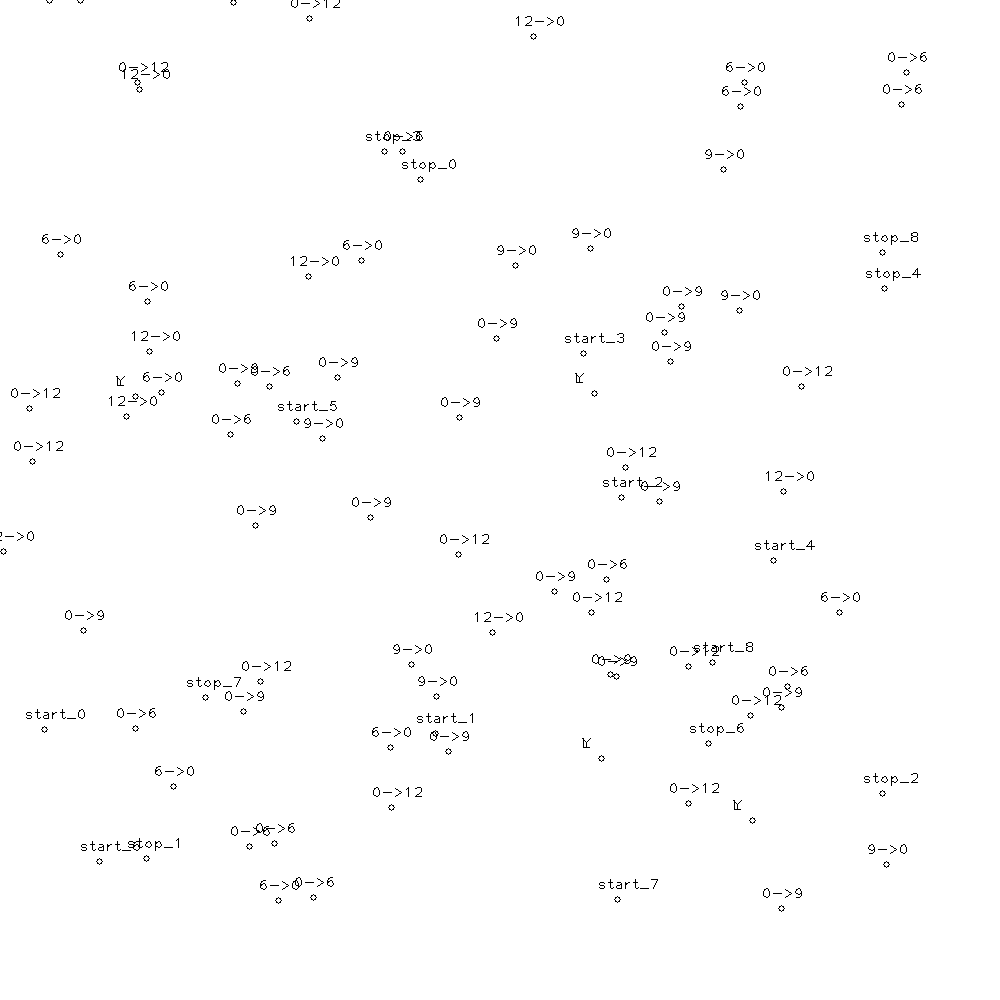
\includegraphics[width=10cm]{images/0_original.png}}

Two alternate solutions are given here.
They are both local minima with respect to a very primitive local neighbor search.
(Which is going to be improved.)

\fbox{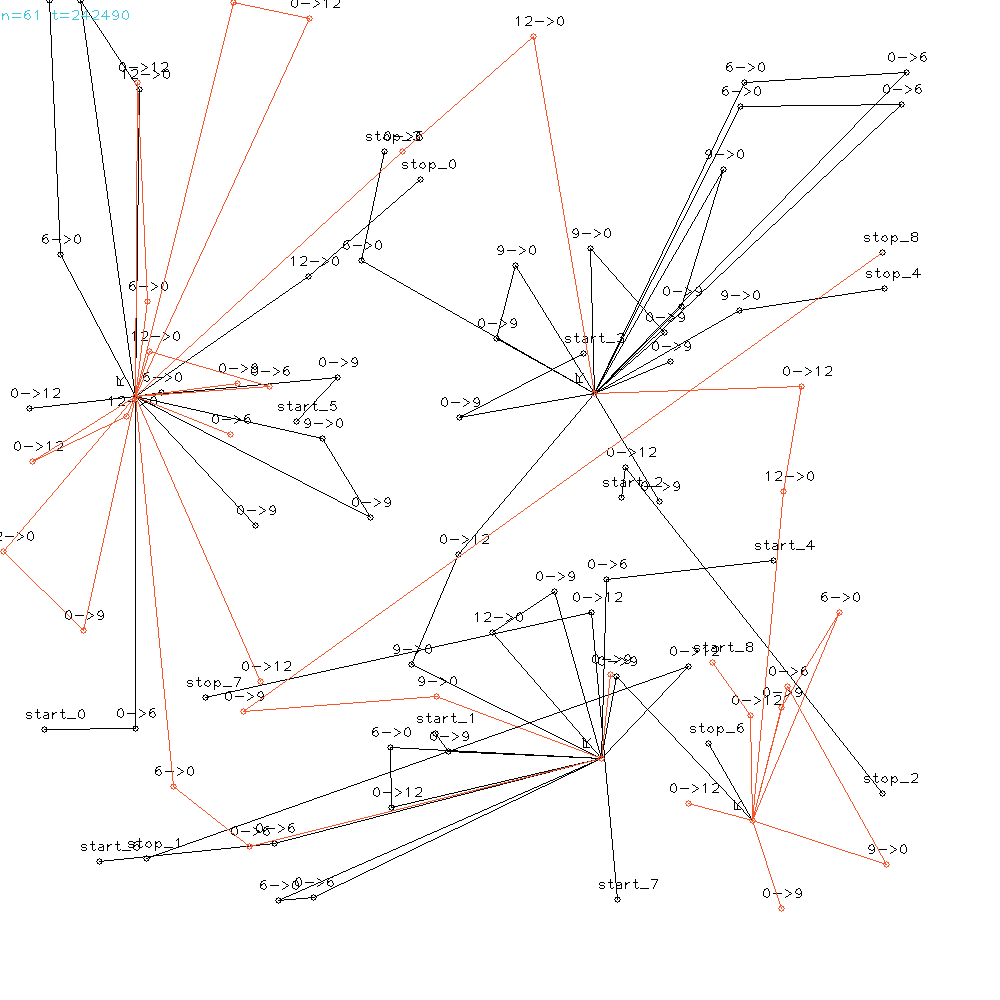
\includegraphics[width=6cm]{images/0_alternate_1.png}}
\fbox{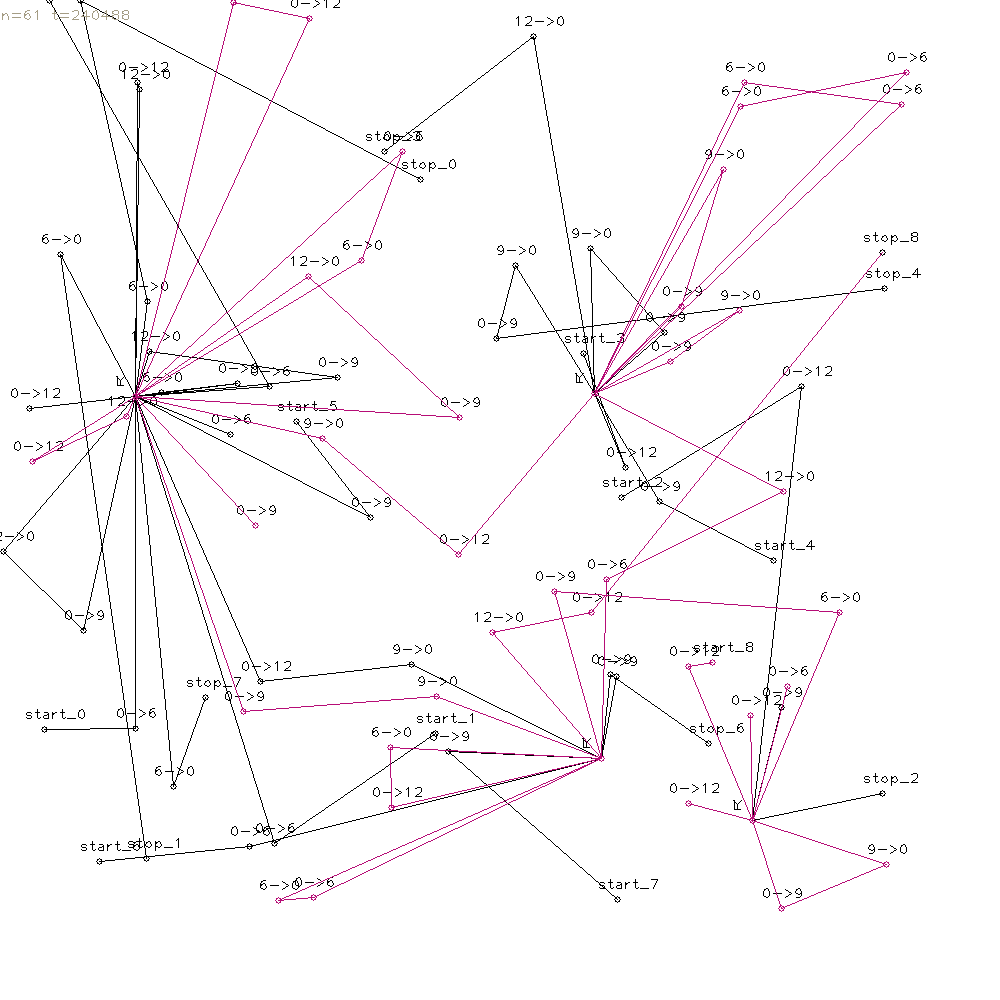
\includegraphics[width=6cm]{images/0_alternate_2.png}}

After cutting the first solution at time $52221$, we applied mutations to the first subcity to get the city on the right from the original subcity on the left.

\fbox{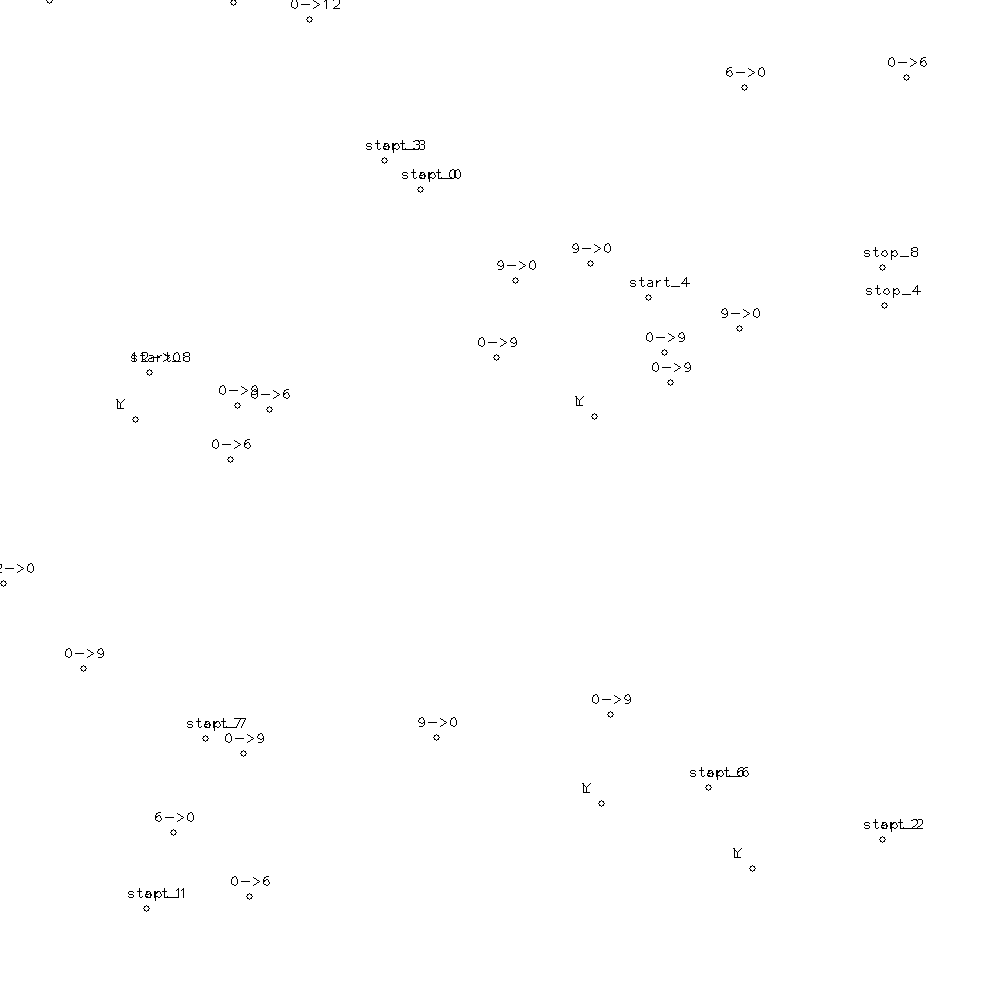
\includegraphics[width=6cm]{images/0_reduced_city_1.png}}
\fbox{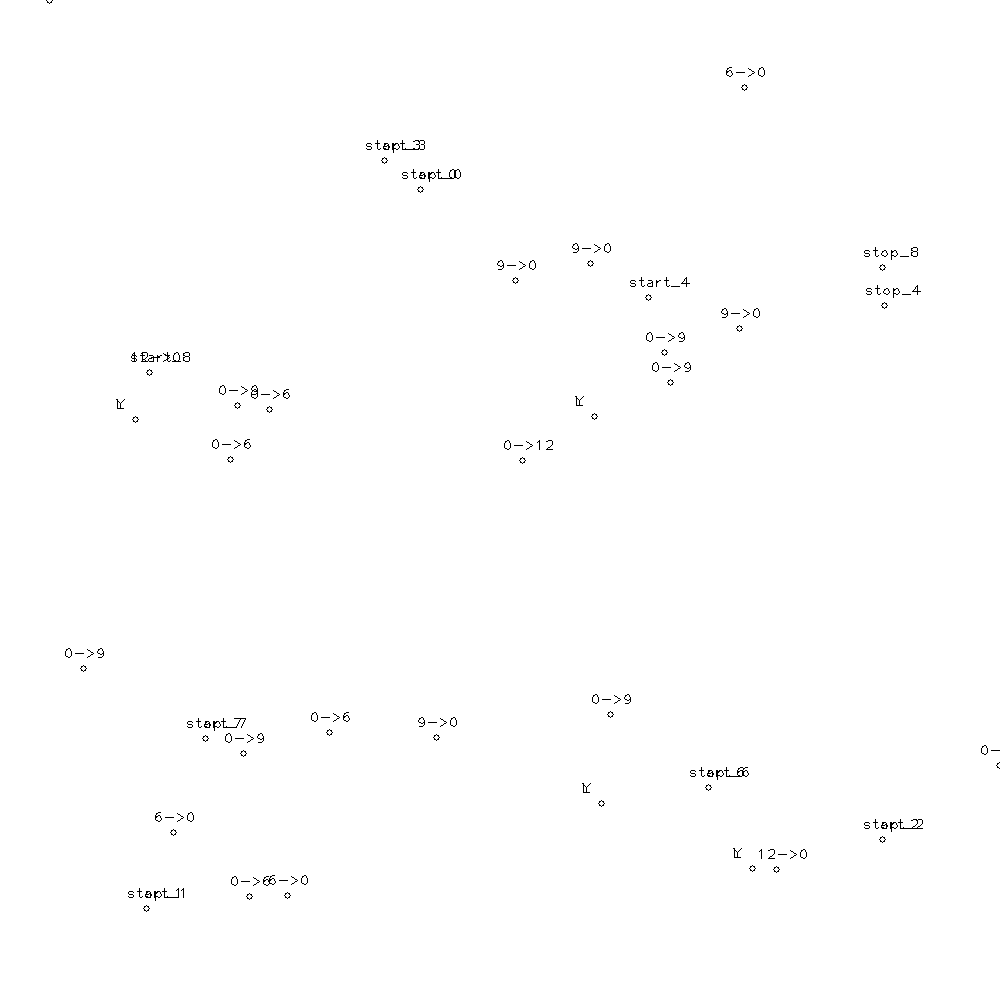
\includegraphics[width=6cm]{images/0_mutated_city_1.png}}

Finally, we have the solutions to the mutated subcities.

\fbox{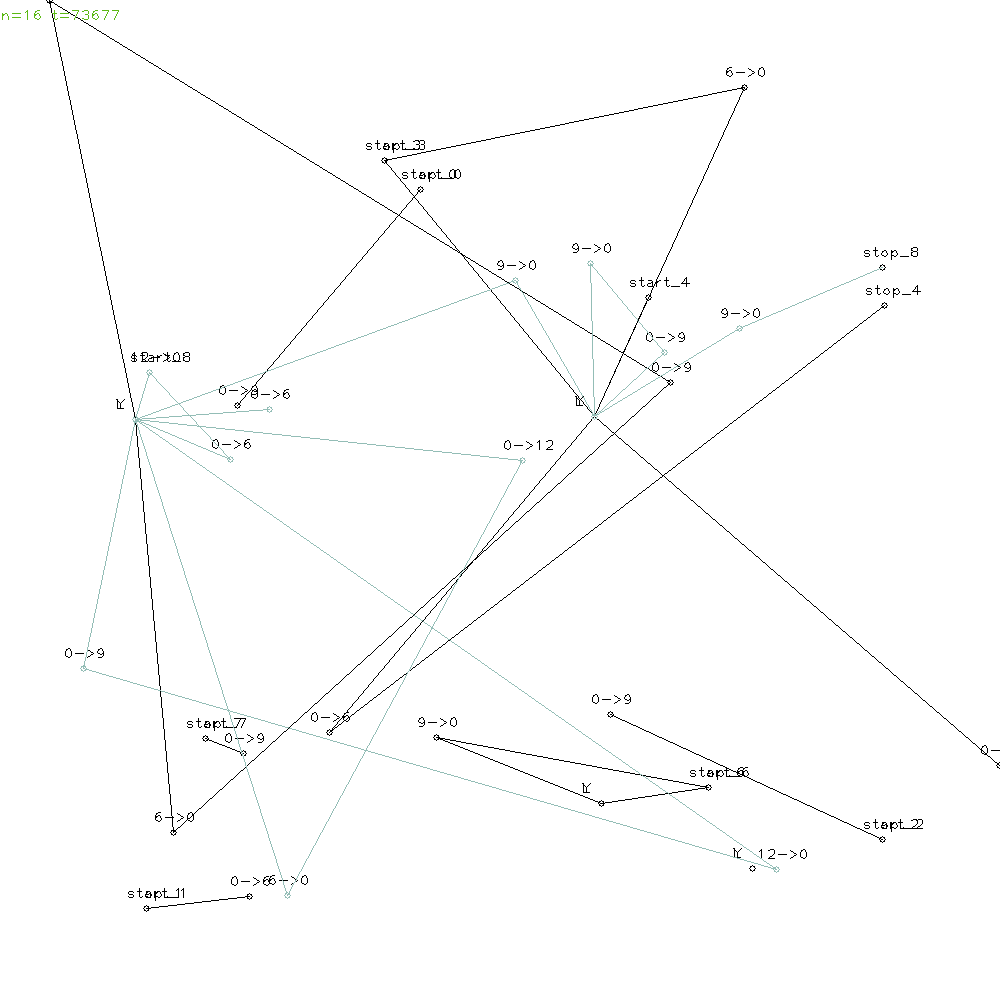
\includegraphics[width=6cm]{images/0_mutated_solution_1.png}}
\fbox{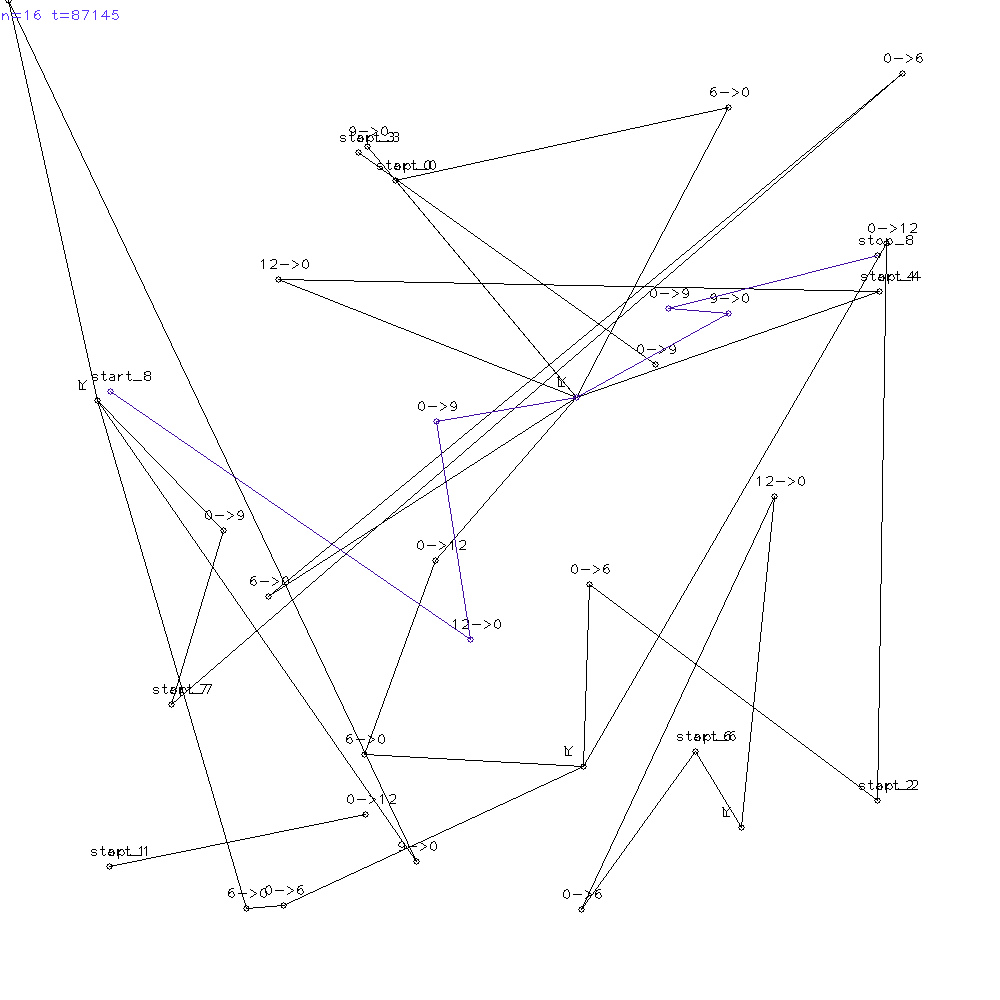
\includegraphics[width=6cm]{images/0_mutated_solution_2.png}}

\subsubsection{Results and Interpretation}
The previous images depict one trial.
For this first trial, the sum of times of all drivers for $s_1$ was $242490$, while the sum for $s_2$ was $240488$.
The minimum of $s_1$ and $s_2$'s maximum driver's drive time was $96188$, and we selected time $52221$ to cut the city into its subcity.
When we solved the problem for the two subcities, we found that the sum of all drive times for the first city was $73677$, while the sum for the second subcity was $87145$.

This process was continued 4 more times to produce the following output, where the previous numbers are shown.
Each bracketed column represents another trial.
\begin{verbatim}
total:
[242490:240488] [236186:243216] [270128:268134] [239330:224200] [232833:234310] 
cut time:
[ 52221: 96188] [ 43933: 78308] [ 72937: 90835] [ 38051: 58019] [ 34193: 61245] 
reduced:
[ 73677: 87145] [ 53775: 91516] [ 19789: 26255] [ 76986: 57646] [ 58588: 58175] 
diff:
[  2002:-13468] [  7030: 37741] [  1994: -6466] [ 15130: 19340] [  1477:  -413] 
\end{verbatim}

\paragraph{Interpretation}
The additional last line is the most important.
It means that although the better ($\min$) of the two alternatives was $2002$ seconds faster than the alternative, the solution to its subcity problem with $t=52221$ was $13468$ \emph{slower} than the solution to the subcity problem for the slower solution.

Out of the $5$ trials that were run, $3$ of the solutions that had faster times for the original city admitted slower times for the subcity problem.
Of course, in each particular case, this could be because the mutations for the subcities forced their solutions to have slower times.
However, with a high number of trials, the differences in mutation should be averaged out.

\paragraph{Drawing Conclusions from Results}
One proposed statistical test could be to see if the variance in subcity solutions from the above process is different from the variance when the two alternate solutions are the same.
This would mean that the variance in subcity solutions for different solutions is different from the variance in subcity drive time caused by the mutation of the subcity.

Another test that may be more natural is to not generate a new city each test.
Rather apply several different mutations and come up with several different times for each initial pair of alternative solutions.
Perhaps, enough tests could be done in order to determine if the mean difference in subcity solutions is $0$.
Then, this inner test would be conducted several times, and we could get a sense of how often solutions have differing robustness.
For example, a solution's robustness may be important if $80$ out of $100$ pairs of solutions had statistically significant differences in the means of their subcity solutions.

Boht of these expirements have non-parametric tests that should be able to determine if robustness as we have defined it varies from solution to solution.
For the first test, we may use Levene's test or the Kolmogorov-Smirnov test, while a Mann-Whitney test could be useful for the second.

\subsubsection{This isn't done yet}
There are several caveats of this process in its current state.
(This is why we haven't ran the statistical test :)

We used the sum of all times, instead of the maximum time, because that is was what our primitive solver optimized.
This problem is already fixed, although the images in this presentation do not reflect this.
The new solver has an objective of num drivers squared times maximum time + sum of all times.
This seems to produces better output than using an overtime penalty based on the sum of times past the minimum driver's time.

Right now, there is a problem that if the driver is waiting at a landfill, with say 20 minutes left after the cutting time, he no longer has to wait that 20 mins in the subcity.
We are not sure if this is worth fixing.

Also, right now a there is a bug with multiple start locations, where if a driver does not service any requests, he does not have to end at the end location.
This is an artifact of trying to define multiple start locations, and will be fixed soon.

Also, currently the driving end states aren't required to have no dumpster.
(These images aren't from the matlab simulator.).
This is already fixed, although the images in this presentation do not reflect this.

Of course, we are comparing random good solutions, without trying to find robust solutions.
The differences might be bigger if we could actually search for robust solutions.
This means we might should take the maximum of differences in robustness, rather than average when determining the usefullness of this concept.


\subsection{Changing Times}
One of the assumptions made in the class was that drive times do not depend on the time of day.
We are currently collecting drive times through different times of days, and hope to test if this assumption is valid or if simulation output changes drastically when we include dynamic drive times.
One simple test would be constructed in the same way as changing the request locations, only rather than simulating a solution part way through, we just see whether some solutions work better with realistic, changing drive times.
Of course, it could simply turn out that all solutions are simply scaled to take longer based on the variance in times through out the day, without some be scaled more than others.

\subsection{Flexible Dumpster Sizes}
One fairly simple modification to the simulator could allow flexible dumpster sizes.
We could expand our model to include multiple actions per request.
The different actions would have different sizes, so that solutions are allowed to deliver a size $9$ dumpster when the request was for a size $6$ dumpster.
Then the constraint on requests not being serviced multiple times would have to be fixed. (insert latex ref here.)
If this means that solutions are much faster, and this is allowed by Sam's Hauling, then it would be a good idea to include this in the algorithm.
We may add penalties to this based on the extra cost of dumping larger dumpsters.
How important this is to solution times obviously depends on what the distribution of dumpster size requests are in the first place.

\section{Conclusion}

(NOT WRITTEN UNTIL THE REST OF THE DOCUMENT IS FINALIZED)


(Could move rest of tutorial into an appendix)

\end{document}
